\chapter{El ciclo celular y la mitosis}\label{ch:g11:cell-cycle-mitosis}

Aplasta la punta de una raíz de cebolla bajo un cubreobjetos, tíñela y
mira: entre cientos de \omterm{def:g10:cells-common-unit:cell}{células} tranquilas con el \omterm{def:g10:cells-common-unit:organelle}{núcleo} redondo, unas
pocas muestran otra cosa --- bastoncillos oscuros en forma de X
reunidos en el centro de la \omterm{def:g10:cells-common-unit:cell}{célula}, o dos juegos de bastoncillos
separados hacia los extremos, o dos \omterm{def:g10:cells-common-unit:organelle}{núcleos} pequeños con una pared que
se forma entre ellos. Estás viendo la división celular sorprendida en
momentos distintos, en un tejido que crece un milímetro al día. Cada
una de esas divisiones entrega dos juegos completos e idénticos de
\omterm{def:g10:universal-dna:information}{cromosomas} a dos \omterm{def:g10:cells-common-unit:cell}{células} hijas. Este capítulo sigue a una \omterm{def:g10:cells-common-unit:cell}{célula} a lo
largo de un ciclo completo y observa de cerca la hora en la que se
reparten los \omterm{def:g10:universal-dna:information}{cromosomas}.

\section{El ciclo celular}

\begin{definition}[Ciclo celular]\label{def:g11:cell-cycle-mitosis:cycle}
El \emph{ciclo celular}\index{ciclo celular} es la sucesión de
acontecimientos que van desde el nacimiento de una \omterm{def:g10:cells-common-unit:cell}{célula}, por
división, hasta su propia división en dos. Comprende la
\emph{interfase}, durante la cual la \omterm{def:g10:cells-common-unit:cell}{célula} crece y copia su \omterm{def:g10:universal-dna:information}{ADN}, y la
\emph{fase M}, durante la cual se divide el \omterm{def:g10:cells-common-unit:organelle}{núcleo}
(\emph{mitosis}\index{mitosis}) y después el \omterm{def:g10:cells-common-unit:cell}{citoplasma}
(\emph{citocinesis}). La interfase tiene tres partes: $\mathrm{G_1}$
(crecimiento), S (\omterm{def:g11:dna-replication:replication}{replicación del ADN}, \cref{ch:g11:dna-replication}) y
$\mathrm{G_2}$ (preparación de la división).
\end{definition}

\begin{omfigure}
\begin{tikzpicture}[font=\small]
  % pie: G1 11h, S 8h, G2 4h, M 1h  (24h) -> angles: G1 165°, S 120°, G2 60°, M 15°
  \fill[omDef!30] (0,0) -- (90:2.2) arc (90:-75:2.2) -- cycle;
  \fill[omProp!35] (0,0) -- (-75:2.2) arc (-75:-195:2.2) -- cycle;
  \fill[omMeth!35] (0,0) -- (-195:2.2) arc (-195:-255:2.2) -- cycle;
  \fill[omThm!50] (0,0) -- (-255:2.2) arc (-255:-270:2.2) -- cycle;
  \draw[thick] (0,0) circle (2.2);
  \foreach \a in {90,-75,-195,-255} \draw[thick] (0,0) -- (\a:2.2);
  \node at (10:1.3) {$\mathrm{G_1}$};
  \node at (-135:1.3) {S};
  \node at (-225:1.35) {$\mathrm{G_2}$};
  \node[anchor=south east] at (-262:2.35) {M};
  \node[anchor=west, align=left] at (2.6,1.3) {$\mathrm{G_1}$: crecimiento, unas \qty{11}{h}};
  \node[anchor=west, align=left] at (2.6,0.5) {S: replicación del ADN, \qty{8}{h}};
  \node[anchor=west, align=left] at (2.6,-0.3) {$\mathrm{G_2}$: preparación, \qty{4}{h}};
  \node[anchor=west, align=left] at (2.6,-1.1) {M: mitosis y citocinesis, \qty{1}{h}};
  \draw[->, thick] (100:2.5) arc (100:130:2.5);
\end{tikzpicture}

{\small El \omterm{def:g11:cell-cycle-mitosis:cycle}{ciclo celular} de una \omterm{def:g10:cells-common-unit:cell}{célula} humana típica en división, de
unas 24 horas. La interfase ($\mathrm{G_1}$, S, $\mathrm{G_2}$) ocupa
23 de ellas; la división misma, una. Muchas \omterm{def:g10:cells-common-unit:cell}{células} salen del ciclo tras
$\mathrm{G_1}$ y no vuelven a dividirse.}
\end{omfigure}

\begin{proposition}[El ADN a lo largo del ciclo]\label{prop:g11:cell-cycle-mitosis:dna}
Llamemos $q$ a la cantidad de \omterm{def:g10:universal-dna:information}{ADN} de un \omterm{def:g10:cells-common-unit:organelle}{núcleo} justo después de una
división. Se mantiene en $q$ durante $\mathrm{G_1}$, sube de forma
sostenida hasta $2q$ durante S mientras se copian los \omterm{def:g10:universal-dna:information}{cromosomas}, se
mantiene en $2q$ durante $\mathrm{G_2}$ y la primera parte de la
\omterm{def:g11:cell-cycle-mitosis:cycle}{mitosis}, y vuelve a bajar a $q$ en cada \omterm{def:g10:cells-common-unit:organelle}{núcleo} hijo al final de la
\omterm{def:g11:cell-cycle-mitosis:cycle}{mitosis}. El número de \omterm{def:g10:universal-dna:information}{cromosomas} no cambia durante S: cada \omterm{def:g11:cell-cycle-mitosis:chromosome}{cromosoma} se
copia en dos \emph{\omterm{def:g11:cell-cycle-mitosis:chromosome}{cromátidas}} idénticas unidas por su
\emph{\omterm{def:g11:cell-cycle-mitosis:chromosome}{centrómero}}, y solo se separa en dos \omterm{def:g10:universal-dna:information}{cromosomas} durante la
\omterm{def:g11:cell-cycle-mitosis:cycle}{mitosis}.
\end{proposition}
\admitted

\begin{omfigure}
\begin{tikzpicture}
\begin{axis}[
  width=0.9\linewidth, height=5.4cm,
  axis x line=bottom, axis y line=left,
  xmin=0, xmax=50, ymin=0, ymax=2.8,
  xlabel={tiempo (h)}, ylabel={ADN por núcleo},
  xlabel style={font=\small, at={(axis description cs:0.5,-0.1)}, anchor=north},
  ylabel style={font=\small},
  tick label style={font=\small}, xtick={0,11,19,23,24,35,43,47,48},
  xticklabels={0,11,19,23,,24,35,43,,48},
  ytick={1,2}, yticklabels={$q$, $2q$},
  clip=false,
]
\addplot[thick, omDef] coordinates {(0,1) (11,1) (19,2) (23,2) (23.9,2) (24,1) (35,1) (43,2) (47,2) (47.9,2) (48,1) (50,1)};
\node[font=\small, anchor=south] at (axis cs:5.5,2.25) {$\mathrm{G_1}$};
\node[font=\small, anchor=south] at (axis cs:15,2.25) {S};
\node[font=\small, anchor=south] at (axis cs:21,2.25) {$\mathrm{G_2}$};
\node[font=\small, anchor=south] at (axis cs:29.5,2.25) {$\mathrm{G_1}$};
\node[font=\small, anchor=south] at (axis cs:39,2.25) {S};
\node[font=\small, anchor=south] at (axis cs:45,2.25) {$\mathrm{G_2}$};
\node[font=\small, anchor=south, omThm] at (axis cs:23.5,2.55) {M};
\node[font=\small, anchor=south, omThm] at (axis cs:47.5,2.55) {M};
\draw[dashed, gray] (axis cs:11,0) -- (axis cs:11,2.2);
\draw[dashed, gray] (axis cs:19,0) -- (axis cs:19,2.2);
\draw[dashed, gray] (axis cs:23,0) -- (axis cs:23,2.2);
\draw[dashed, gray] (axis cs:24,0) -- (axis cs:24,2.2);
\draw[dashed, gray] (axis cs:35,0) -- (axis cs:35,2.2);
\draw[dashed, gray] (axis cs:43,0) -- (axis cs:43,2.2);
\draw[dashed, gray] (axis cs:47,0) -- (axis cs:47,2.2);
\end{axis}
\end{tikzpicture}

{\small Cantidad de \omterm{def:g10:universal-dna:information}{ADN} de un \omterm{def:g10:cells-common-unit:organelle}{núcleo} a lo largo de dos ciclos
sucesivos de 24 horas. Se duplica durante S y se reduce a la mitad al
final de la \omterm{def:g11:cell-cycle-mitosis:cycle}{mitosis}; una \omterm{def:g10:cells-common-unit:cell}{célula} hija empieza siempre con $q$.}
\end{omfigure}

\begin{example}[Leer la curva]\label{ex:g11:cell-cycle-mitosis:reading}
Una \omterm{def:g10:cells-common-unit:cell}{célula} medida en $2q$ puede estar en $\mathrm{G_2}$ o al principio
de la \omterm{def:g11:cell-cycle-mitosis:cycle}{mitosis}; en $1.5q$ está sin duda en S, a mitad de la replicación;
en $q$ está en $\mathrm{G_1}$ --- o ha salido del ciclo para siempre,
como una neurona o una fibra muscular, que se quedan en $q$ de por
vida. Un tejido en el que todas las \omterm{def:g10:cells-common-unit:cell}{células} están en $q$ es un tejido
que ha dejado de dividirse.
\end{example}

\section{Los cromosomas, vistos}

\begin{definition}[Cromosoma, cromátida, cariotipo]\label{def:g11:cell-cycle-mitosis:chromosome}
Un \emph{cromosoma} es una molécula de \omterm{def:g10:universal-dna:information}{ADN} con sus \omterm{def:g10:chemistry-of-life:families}{proteínas} de
empaquetamiento. Entre dos divisiones es un hilo suelto e invisible; al
principio de la \omterm{def:g11:cell-cycle-mitosis:cycle}{mitosis} se pliega en un bastoncillo compacto visible al
microscopio óptico. Tras la replicación, cada cromosoma consta de dos
\emph{cromátidas}\index{cromátida} idénticas, unidas por el
\emph{centrómero}\index{centrómero}: la conocida forma de X. El
\emph{cariotipo}\index{cariotipo} de una \omterm{def:g10:biodiversity-scales:species}{especie} es su juego completo
de \omterm{def:g10:universal-dna:information}{cromosomas}, fotografiado en metafase y ordenado por parejas según el
tamaño: una \omterm{def:g10:cells-common-unit:cell}{célula} humana tiene 46, en 23 parejas, y los dos miembros
de una pareja son \emph{homólogos} --- mismos \omterm{def:g10:universal-dna:gene}{genes} en las mismas
posiciones, uno de cada progenitor.
\end{definition}

\begin{omfigure}
\begin{tikzpicture}[font=\scriptsize, line cap=round]
  % 22 autosome pairs of decreasing size, then X and Y; each chromosome = two chromatids
  \tikzset{chrom/.style={line width=2.6pt, omDef!75}}
  \foreach \n/\h/\c in {1/2.4/0.55, 2/2.3/0.5, 3/2.0/0.5, 4/1.9/0.35, 5/1.8/0.35, 6/1.7/0.45, 7/1.55/0.42, 8/1.45/0.4}
    { \pgfmathsetmacro{\x}{(\n-1)*1.55}
      \draw[chrom] (\x,0) -- (\x,\h); \draw[chrom] (\x+0.22,0) -- (\x+0.22,\h);
      \fill[omThm] (\x+0.11,{\h*\c}) circle (2pt);
      \node[anchor=north] at (\x+0.11,-0.08) {\n}; }
  \foreach \n/\h/\c in {9/1.4/0.35, 10/1.35/0.35, 11/1.35/0.4, 12/1.3/0.3, 13/1.1/0.15, 14/1.05/0.15, 15/1.0/0.15, 16/0.9/0.45}
    { \pgfmathsetmacro{\x}{(\n-9)*1.55}
      \draw[chrom] (\x,-3.2) -- (\x,-3.2+\h); \draw[chrom] (\x+0.22,-3.2) -- (\x+0.22,-3.2+\h);
      \fill[omThm] (\x+0.11,{-3.2+\h*\c}) circle (2pt);
      \node[anchor=north] at (\x+0.11,-3.28) {\n}; }
  \foreach \n/\h/\c in {17/0.85/0.3, 18/0.8/0.2, 19/0.65/0.5, 20/0.65/0.5, 21/0.5/0.2, 22/0.5/0.2}
    { \pgfmathsetmacro{\x}{(\n-17)*1.55}
      \draw[chrom] (\x,-5.6) -- (\x,-5.6+\h); \draw[chrom] (\x+0.22,-5.6) -- (\x+0.22,-5.6+\h);
      \fill[omThm] (\x+0.11,{-5.6+\h*\c}) circle (2pt);
      \node[anchor=north] at (\x+0.11,-5.68) {\n}; }
  % sex chromosomes
  \draw[chrom] (9.3,-5.6) -- (9.3,-4.1); \draw[chrom] (9.52,-5.6) -- (9.52,-4.1); \fill[omThm] (9.41,-4.85) circle (2pt);
  \node[anchor=north] at (9.41,-5.68) {X};
  \draw[chrom] (10.85,-5.6) -- (10.85,-5.1); \draw[chrom] (11.07,-5.6) -- (11.07,-5.1); \fill[omThm] (10.96,-5.5) circle (2pt);
  \node[anchor=north] at (10.96,-5.68) {Y};
\end{tikzpicture}

{\small Un \omterm{def:g11:cell-cycle-mitosis:chromosome}{cariotipo} humano, en esquema: las 22 parejas de \omterm{def:g10:universal-dna:information}{cromosomas}
corrientes numeradas por tamaño decreciente y, después, los \omterm{def:g10:universal-dna:information}{cromosomas}
sexuales --- aquí X e Y, así que es un varón. Cada \omterm{def:g11:cell-cycle-mitosis:chromosome}{cromosoma} está
dibujado con sus dos \omterm{def:g11:cell-cycle-mitosis:chromosome}{cromátidas} y el \omterm{def:g11:cell-cycle-mitosis:chromosome}{centrómero} en rojo.}
\end{omfigure}

\begin{omfigure}
\begin{tikzpicture}[font=\small, line cap=round]
  % single chromatid chromosome
  \draw[line width=5pt, omDef!70] (0,-1.2) -- (0,1.2);
  \fill[omThm] (0,0.2) circle (3.5pt);
  \node[anchor=north, align=center] at (0,-1.5) {antes de la fase S:\\ una cromátida};
  % arrow
  \draw[->, thick] (1.2,0) -- (2.6,0) node[midway, above] {S};
  % two chromatid chromosome
  \draw[line width=5pt, omDef!70] (3.6,-1.2) .. controls (3.75,-0.3) and (3.75,0.3) .. (3.6,1.2);
  \draw[line width=5pt, omDef!70] (4.2,-1.2) .. controls (4.05,-0.3) and (4.05,0.3) .. (4.2,1.2);
  \fill[omThm] (3.9,0.2) circle (3.5pt);
  \node[anchor=north, align=center] at (3.9,-1.5) {tras la fase S:\\ dos cromátidas idénticas};
  \draw[->] (5.6,0.2) -- (4.15,0.2) node[pos=0, anchor=west] {centrómero};
  \draw[->] (5.6,0.9) -- (4.35,0.9) node[pos=0, anchor=west] {cromátida};
  % after anaphase
  \draw[->, thick] (8.6,0) -- (10.0,0) node[midway, above] {anafase};
  \draw[line width=5pt, omDef!70] (10.8,-1.2) -- (10.8,1.2);
  \fill[omThm] (10.8,0.2) circle (3.5pt);
  \draw[line width=5pt, omDef!70] (11.8,-1.2) -- (11.8,1.2);
  \fill[omThm] (11.8,0.2) circle (3.5pt);
  \node[anchor=north, align=center] at (11.3,-1.5) {dos cromosomas,\\ uno para cada célula};
\end{tikzpicture}

{\small Un \omterm{def:g11:cell-cycle-mitosis:chromosome}{cromosoma} a lo largo del ciclo. La replicación lo convierte
en dos \omterm{def:g11:cell-cycle-mitosis:chromosome}{cromátidas} unidas por el \omterm{def:g11:cell-cycle-mitosis:chromosome}{centrómero}; la anafase las separa en
dos \omterm{def:g10:universal-dna:information}{cromosomas} de una sola \omterm{def:g11:cell-cycle-mitosis:chromosome}{cromátida}, uno para cada \omterm{def:g10:cells-common-unit:cell}{célula} hija. El
recuento de \omterm{def:g10:universal-dna:information}{cromosomas} solo cambia en la anafase.}
\end{omfigure}

\section{La mitosis, paso a paso}

\begin{proposition}[Las cuatro etapas de la mitosis]\label{prop:g11:cell-cycle-mitosis:stages}
La \omterm{def:g11:cell-cycle-mitosis:cycle}{mitosis} es un movimiento continuo, que se describe en cuatro etapas.
\begin{enumerate}
  \item \emph{Profase}: los \omterm{def:g10:universal-dna:information}{cromosomas} se condensan en bastoncillos
        visibles de dos \omterm{def:g11:cell-cycle-mitosis:chromosome}{cromátidas}; la envoltura nuclear se deshace; se
        forma un \emph{huso} de fibras proteicas entre los dos polos de
        la \omterm{def:g10:cells-common-unit:cell}{célula}.
  \item \emph{Metafase}: los \omterm{def:g10:universal-dna:information}{cromosomas}, unidos a las fibras del huso
        por sus \omterm{def:g11:cell-cycle-mitosis:chromosome}{centrómeros}, se alinean en el plano ecuatorial de la
        \omterm{def:g10:cells-common-unit:cell}{célula}.
  \item \emph{Anafase}: los \omterm{def:g11:cell-cycle-mitosis:chromosome}{centrómeros} se dividen; las dos \omterm{def:g11:cell-cycle-mitosis:chromosome}{cromátidas}
        de cada \omterm{def:g11:cell-cycle-mitosis:chromosome}{cromosoma}, ahora dos \omterm{def:g10:universal-dna:information}{cromosomas}, son arrastradas a
        polos opuestos por las fibras que se acortan.
  \item \emph{Telofase}: una envoltura nuclear vuelve a formarse
        alrededor de cada juego; los \omterm{def:g10:universal-dna:information}{cromosomas} se desenrollan. La
        citocinesis divide después el \omterm{def:g10:cells-common-unit:cell}{citoplasma} --- estrangulándolo en
        las \omterm{def:g10:cells-common-unit:cell}{células} animales, construyendo una pared nueva en las
        vegetales.
\end{enumerate}
Cada \omterm{def:g10:cells-common-unit:cell}{célula} hija recibe una \omterm{def:g11:cell-cycle-mitosis:chromosome}{cromátida} de cada \omterm{def:g11:cell-cycle-mitosis:chromosome}{cromosoma}: el mismo
número de \omterm{def:g10:universal-dna:information}{cromosomas} que la madre, con el mismo \omterm{def:g10:universal-dna:information}{ADN}.
\end{proposition}
\admitted

\begin{omfigure}
\begin{tikzpicture}[font=\small, line cap=round]
  \tikzset{cellb/.style={draw, thick, fill=omDef!5, rounded corners=10pt, minimum width=2.9cm, minimum height=2.6cm},
           chr/.style={line width=3pt, omDef!80}, cen/.style={fill=omThm}}
  % prophase
  \begin{scope}
    \node[cellb] at (0,0) {};
    \draw[thick, dashed, gray] (0,0) circle (0.95);
    \draw[chr] (-0.5,0.5) .. controls (-0.35,0.1) .. (-0.5,-0.3); \draw[chr] (-0.2,0.5) .. controls (-0.35,0.1) .. (-0.2,-0.3); \fill[cen] (-0.35,0.1) circle (2pt);
    \draw[chr] (0.2,0.6) .. controls (0.35,0.2) .. (0.2,-0.2); \draw[chr] (0.5,0.6) .. controls (0.35,0.2) .. (0.5,-0.2); \fill[cen] (0.35,0.2) circle (2pt);
    \node[anchor=north, align=center] at (0,-1.45) {profase};
  \end{scope}
  % metaphase
  \begin{scope}[xshift=3.6cm]
    \node[cellb] at (0,0) {};
    \fill (0,1.1) circle (2pt); \fill (0,-1.1) circle (2pt);
    \foreach \x in {-0.45,0.45} { \draw[gray] (0,1.1) -- (\x,0.05); \draw[gray] (0,-1.1) -- (\x,-0.05); }
    \foreach \x in {-0.45,0.45} {
      \draw[chr] (\x-0.13,0.55) .. controls (\x,0.0) .. (\x-0.13,-0.55);
      \draw[chr] (\x+0.13,0.55) .. controls (\x,0.0) .. (\x+0.13,-0.55);
      \fill[cen] (\x,0) circle (2pt);
    }
    \draw[dashed, gray] (-1.3,0) -- (1.3,0);
    \node[anchor=north, align=center] at (0,-1.45) {metafase};
  \end{scope}
  % anaphase
  \begin{scope}[xshift=7.2cm]
    \node[cellb] at (0,0) {};
    \fill (0,1.1) circle (2pt); \fill (0,-1.1) circle (2pt);
    \foreach \x in {-0.45,0.45} { \draw[gray] (0,1.1) -- (\x,0.6); \draw[gray] (0,-1.1) -- (\x,-0.6); }
    \foreach \x in {-0.45,0.45} {
      \draw[chr] (\x,0.6) .. controls (\x-0.1,0.4) .. (\x-0.25,0.05);
      \draw[chr] (\x,0.6) .. controls (\x+0.1,0.4) .. (\x+0.25,0.05);
      \fill[cen] (\x,0.6) circle (2pt);
      \draw[chr] (\x,-0.6) .. controls (\x-0.1,-0.4) .. (\x-0.25,-0.05);
      \draw[chr] (\x,-0.6) .. controls (\x+0.1,-0.4) .. (\x+0.25,-0.05);
      \fill[cen] (\x,-0.6) circle (2pt);
    }
    \node[anchor=north, align=center] at (0,-1.45) {anafase};
  \end{scope}
  % telophase
  \begin{scope}[xshift=10.8cm]
    \draw[thick, fill=omDef!5] (-1.45,1.3) .. controls (-1.6,0.3) and (-0.3,0.3) .. (0,0) .. controls (-0.3,-0.3) and (-1.6,-0.3) .. (-1.45,-1.3) -- cycle;
    \draw[thick, fill=omDef!5] (1.45,1.3) .. controls (1.6,0.3) and (0.3,0.3) .. (0,0) .. controls (0.3,-0.3) and (1.6,-0.3) .. (1.45,-1.3) -- cycle;
    \draw[thick, fill=omDef!5, rounded corners=10pt] (-1.45,-1.3) rectangle (1.45,1.3);
    \draw[thick, fill=white] (-1.45,1.3) .. controls (-1.6,0.3) and (-0.3,0.3) .. (0,0) .. controls (-0.3,-0.3) and (-1.6,-0.3) .. (-1.45,-1.3);
    \draw[thick, fill=white] (1.45,1.3) .. controls (1.6,0.3) and (0.3,0.3) .. (0,0) .. controls (0.3,-0.3) and (1.6,-0.3) .. (1.45,-1.3);
    \draw[thick, dashed, gray] (-0.75,0) circle (0.5); \draw[thick, dashed, gray] (0.75,0) circle (0.5);
    \foreach \x in {-0.9,-0.6,0.6,0.9} \draw[chr] (\x,0.25) -- (\x,-0.25);
    \node[anchor=north, align=center] at (0,-1.45) {telofase y\\ citocinesis};
  \end{scope}
\end{tikzpicture}

{\small \omterm{def:g11:cell-cycle-mitosis:cycle}{Mitosis} de una \omterm{def:g10:cells-common-unit:cell}{célula} con dos \omterm{def:g10:universal-dna:information}{cromosomas} ($2n = 2$), cada uno
formado ya por dos \omterm{def:g11:cell-cycle-mitosis:chromosome}{cromátidas}. Profase: condensación, envoltura
deshecha. Metafase: alineación en el ecuador, \omterm{def:g11:cell-cycle-mitosis:chromosome}{centrómeros} unidos al
huso. Anafase: \omterm{def:g11:cell-cycle-mitosis:chromosome}{cromátidas} arrastradas a los polos. Telofase: se rehacen
dos \omterm{def:g10:cells-common-unit:organelle}{núcleos} y la \omterm{def:g10:cells-common-unit:cell}{célula} se divide.}
\end{omfigure}

\begin{omfigure}
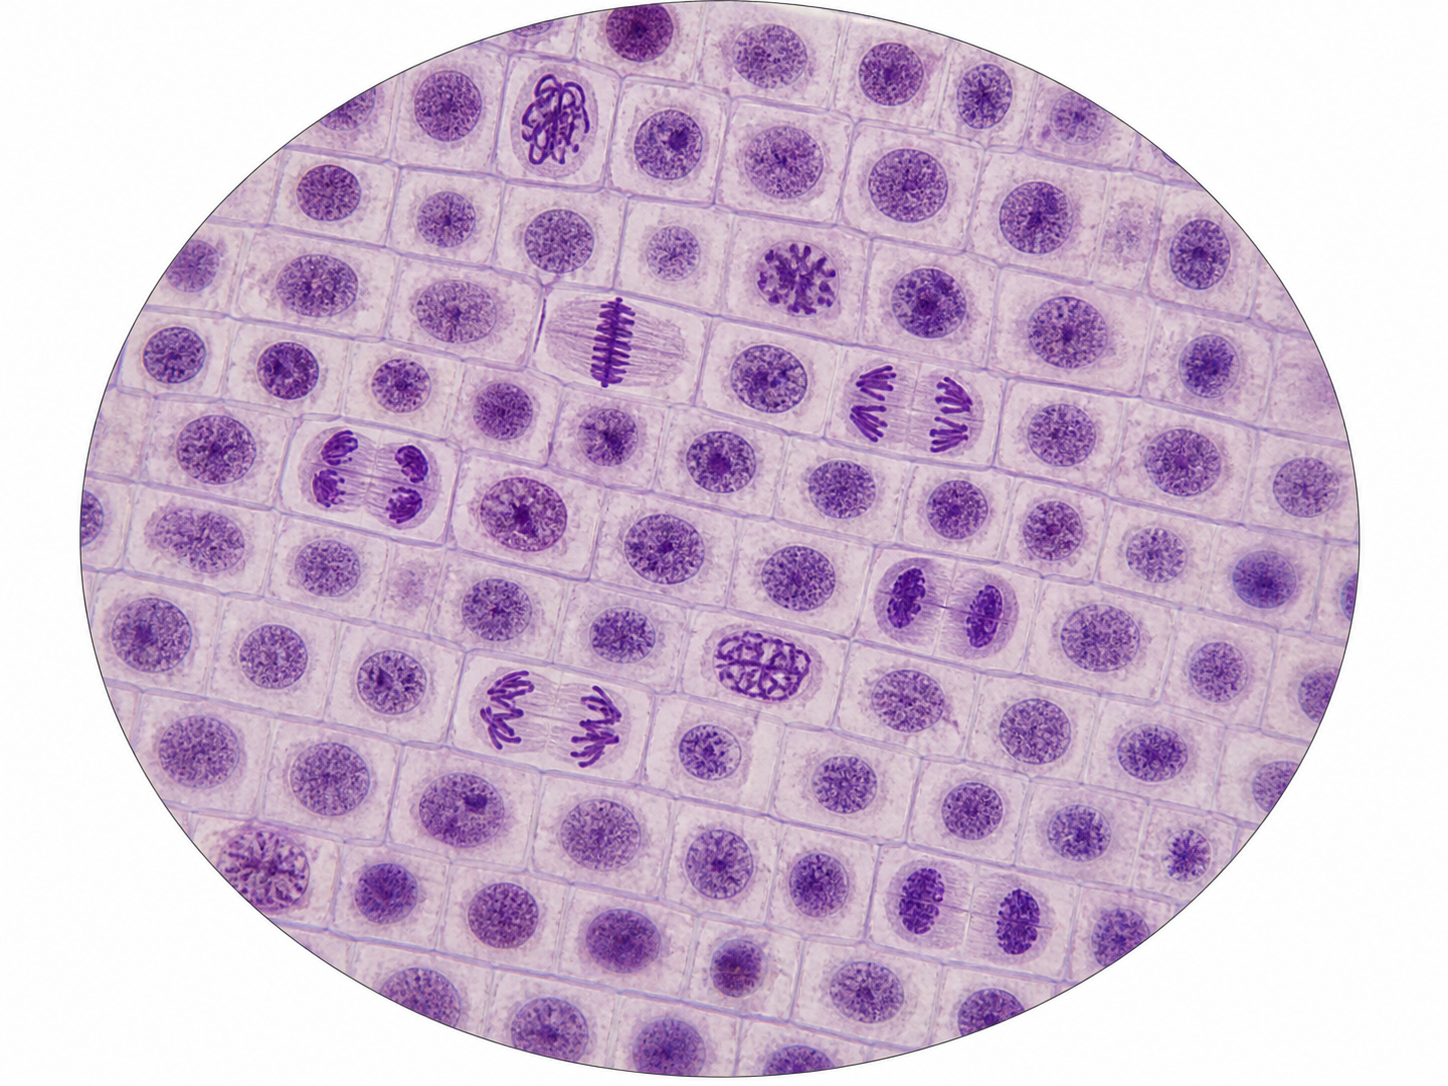
\includegraphics[width=0.58\linewidth]{images/book2/ai/g11-mitosis-root-tip.png}

{\small Un aplastado de punta de raíz de cebolla al microscopio
óptico. Casi todas las \omterm{def:g10:cells-common-unit:cell}{células} están en interfase; unas pocas muestran
\omterm{def:g10:universal-dna:information}{cromosomas} condensados en distintas etapas de la \omterm{def:g11:cell-cycle-mitosis:cycle}{mitosis}. Contar la
proporción de cada etapa mide cuánto dura cada una.}
\end{omfigure}

\begin{example}[Contar en la punta de la raíz]\label{ex:g11:cell-cycle-mitosis:count}
De 600 \omterm{def:g10:cells-common-unit:cell}{células} contadas en una punta de raíz, 540 están en interfase y
60 en \omterm{def:g11:cell-cycle-mitosis:cycle}{mitosis}: un \emph{índice mitótico} del 10\%. Si el ciclo dura 20
horas, la \omterm{def:g11:cell-cycle-mitosis:cycle}{mitosis} dura unas $0.10 \times 20 = \qty{2}{h}$; y si 36 de
las 60 \omterm{def:g10:cells-common-unit:cell}{células} en división están en profase, la profase ocupa $36/60$
de esas dos horas, unos 72 minutos, mientras que la anafase, vista
solo en 4 \omterm{def:g10:cells-common-unit:cell}{células}, dura unos 8 minutos. La etapa más rara es la más
rápida.
\end{example}

\begin{method}[Contar cromosomas y cromátidas]\label{met:g11:cell-cycle-mitosis:counting}
Para una \omterm{def:g10:biodiversity-scales:species}{especie} con $2n$ \omterm{def:g10:universal-dna:information}{cromosomas}:
\begin{enumerate}
  \item en $\mathrm{G_1}$: $2n$ \omterm{def:g10:universal-dna:information}{cromosomas}, con una \omterm{def:g11:cell-cycle-mitosis:chromosome}{cromátida} cada uno,
        \omterm{def:g10:universal-dna:information}{ADN} $q$;
  \item tras S, durante $\mathrm{G_2}$, la profase y la metafase: $2n$
        \omterm{def:g10:universal-dna:information}{cromosomas}, con dos \omterm{def:g11:cell-cycle-mitosis:chromosome}{cromátidas} cada uno ($4n$ \omterm{def:g11:cell-cycle-mitosis:chromosome}{cromátidas}), \omterm{def:g10:universal-dna:information}{ADN}
        $2q$;
  \item a partir de la anafase: $4n$ \omterm{def:g10:universal-dna:information}{cromosomas} de una sola \omterm{def:g11:cell-cycle-mitosis:chromosome}{cromátida}
        en la \omterm{def:g10:cells-common-unit:cell}{célula}, $2n$ camino de cada polo;
  \item en cada \omterm{def:g10:cells-common-unit:cell}{célula} hija: $2n$ \omterm{def:g10:universal-dna:information}{cromosomas}, con una \omterm{def:g11:cell-cycle-mitosis:chromosome}{cromátida} cada
        uno, \omterm{def:g10:universal-dna:information}{ADN} $q$.
\end{enumerate}
Una \omterm{def:g11:cell-cycle-mitosis:chromosome}{cromátida} se convierte en \omterm{def:g11:cell-cycle-mitosis:chromosome}{cromosoma} en el momento en que su
\omterm{def:g11:cell-cycle-mitosis:chromosome}{centrómero} se divide.
\end{method}

\begin{example}[Las cifras humanas]\label{ex:g11:cell-cycle-mitosis:human}
Una \omterm{def:g10:cells-common-unit:cell}{célula} humana en metafase tiene 46 \omterm{def:g10:universal-dna:information}{cromosomas} y 92 \omterm{def:g11:cell-cycle-mitosis:chromosome}{cromátidas}; en
anafase, 92 \omterm{def:g10:universal-dna:information}{cromosomas}, 46 en camino a cada polo; cada hija, 46
\omterm{def:g10:universal-dna:information}{cromosomas} de una \omterm{def:g11:cell-cycle-mitosis:chromosome}{cromátida} cada uno, con exactamente el \omterm{def:g10:universal-dna:information}{ADN} que tenía
la madre al principio de su ciclo.
\end{example}

\section{Para qué sirve la mitosis}

\begin{proposition}[La conformidad y sus usos]\label{prop:g11:cell-cycle-mitosis:conformity}
Como la replicación es fiel y la \omterm{def:g11:cell-cycle-mitosis:cycle}{mitosis} reparte las \omterm{def:g11:cell-cycle-mitosis:chromosome}{cromátidas} con
exactitud, todas las \omterm{def:g10:cells-common-unit:cell}{células} de un cuerpo pluricelular llevan la misma
\omterm{def:g10:universal-dna:information}{información genética} que el óvulo fecundado del que descienden. La
\omterm{def:g11:cell-cycle-mitosis:cycle}{mitosis} es el mecanismo del crecimiento (el embrión, la punta de la
raíz), de la renovación (la piel, el revestimiento intestinal, la
sangre: solo la médula ósea fabrica unas $\num{2e11}$ \omterm{def:g10:cells-common-unit:cell}{células} al día) y
de la reparación (la cicatrización de una herida); en los eucariotas
unicelulares es la reproducción misma. Su control --- la decisión de
entrar en el ciclo, las comprobaciones antes de S y antes de la
anafase --- es el tema del \cref{ch:g11:cancer}.
\end{proposition}
\admitted

\begin{remark}[No todo se divide]\label{rem:g11:cell-cycle-mitosis:notall}
Casi todas las neuronas y las \omterm{def:g10:cells-common-unit:cell}{células} del músculo cardíaco salen del
ciclo en la primera infancia y no vuelven a entrar en él: su daño no se
repara por división, y por eso una lesión medular o un infarto dejan
una pérdida permanente. Las \omterm{def:g10:cells-common-unit:cell}{células} del hígado descansan en
$\mathrm{G_1}$ durante meses, pero vuelven a entrar en el ciclo cuando
se extirpa parte del hígado, y regeneran el órgano en unas semanas. Qué
\omterm{def:g10:cells-common-unit:cell}{células} pueden dividirse, y cuándo, es una de las regulaciones más
estrictas del cuerpo.
\end{remark}

\section{Ejercicios}

\begin{exercise}[$\star$]\label{exo:g11:cell-cycle-mitosis:1}
Nombra las cuatro fases del \omterm{def:g11:cell-cycle-mitosis:cycle}{ciclo celular} y di qué ocurre en cada una.
\end{exercise}

\begin{exercise}[$\star$]\label{exo:g11:cell-cycle-mitosis:2}
Define \omterm{def:g11:cell-cycle-mitosis:chromosome}{cromátida} y \omterm{def:g11:cell-cycle-mitosis:chromosome}{centrómero}. ¿Cuándo tiene dos \omterm{def:g11:cell-cycle-mitosis:chromosome}{cromátidas} un
\omterm{def:g11:cell-cycle-mitosis:chromosome}{cromosoma}?
\end{exercise}

\begin{exercise}[$\star$]\label{exo:g11:cell-cycle-mitosis:3}
Enumera las cuatro etapas de la \omterm{def:g11:cell-cycle-mitosis:cycle}{mitosis} con un acontecimiento clave de
cada una.
\end{exercise}

\begin{exercise}[$\star$]\label{exo:g11:cell-cycle-mitosis:4}
Un \omterm{def:g10:cells-common-unit:organelle}{núcleo} contiene $1.5q$ de \omterm{def:g10:universal-dna:information}{ADN}. ¿En qué fase está la \omterm{def:g10:cells-common-unit:cell}{célula}?
\end{exercise}

\begin{exercise}[$\star$]\label{exo:g11:cell-cycle-mitosis:5}
¿Cuántos \omterm{def:g10:universal-dna:information}{cromosomas} y cuántas \omterm{def:g11:cell-cycle-mitosis:chromosome}{cromátidas} tiene una \omterm{def:g10:cells-common-unit:cell}{célula} humana en
$\mathrm{G_2}$?
\end{exercise}

\begin{exercise}[$\star\star$]\label{exo:g11:cell-cycle-mitosis:6}
Con la figura de la cantidad de \omterm{def:g10:universal-dna:information}{ADN}, da la duración de cada fase y di
en qué fases se encontraría una \omterm{def:g10:cells-common-unit:cell}{célula} con $2q$.
\end{exercise}

\begin{exercise}[$\star\star$]\label{exo:g11:cell-cycle-mitosis:7}
Un ratón tiene $2n = 40$. Da el número de \omterm{def:g10:universal-dna:information}{cromosomas} y de \omterm{def:g11:cell-cycle-mitosis:chromosome}{cromátidas} de
una \omterm{def:g10:cells-common-unit:cell}{célula} en metafase, en anafase (\omterm{def:g10:cells-common-unit:cell}{célula} entera) y en una \omterm{def:g10:cells-common-unit:cell}{célula}
hija.
\end{exercise}

\begin{exercise}[$\star\star$]\label{exo:g11:cell-cycle-mitosis:8}
En una punta de raíz se cuentan 800 \omterm{def:g10:cells-common-unit:cell}{células}: 720 en interfase, 48 en
profase, 16 en metafase, 6 en anafase y 10 en telofase. Calcula el
índice mitótico y, para un ciclo de 24 horas, la duración de cada
etapa.
\end{exercise}

\begin{exercise}[$\star\star$]\label{exo:g11:cell-cycle-mitosis:9}
La colchicina, un fármaco extraído del cólquico, impide que se forme el
huso. Predice qué le ocurre a una \omterm{def:g10:cells-common-unit:cell}{célula} en división tratada con ella y
por qué los biólogos la usan para preparar \omterm{def:g11:cell-cycle-mitosis:chromosome}{cariotipos}.
\end{exercise}

\begin{exercise}[$\star\star$]\label{exo:g11:cell-cycle-mitosis:10}
Explica por qué los \omterm{def:g10:universal-dna:information}{cromosomas} deben condensarse antes de moverse, y
por qué vuelven a desenrollarse después.
\end{exercise}

\begin{exercise}[$\star\star$]\label{exo:g11:cell-cycle-mitosis:11}
Un óvulo fecundado se divide cada 12 horas los primeros días. ¿Cuántas
\omterm{def:g10:cells-common-unit:cell}{células} hay al cabo de 5 días? ¿Necesitaría cada división una
$\mathrm{G_1}$ completa?
\end{exercise}

\begin{exercise}[$\star\star\star$]\label{exo:g11:cell-cycle-mitosis:12}
En la anafase, las dos \omterm{def:g11:cell-cycle-mitosis:chromosome}{cromátidas} de un \omterm{def:g11:cell-cycle-mitosis:chromosome}{cromosoma} no se separan y las
dos van al mismo polo. Describe las dos \omterm{def:g10:cells-common-unit:cell}{células} hijas (número de
\omterm{def:g10:universal-dna:information}{cromosomas}, \omterm{def:g10:universal-dna:information}{ADN}) y explica por qué un error así, en una \omterm{def:g10:cells-common-unit:cell}{célula} del
cuerpo, no suele tener consecuencias y en algunos casos sí es grave.
\end{exercise}

\begin{exercise}[$\star\star\star$]\label{exo:g11:cell-cycle-mitosis:13}
La médula ósea fabrica $\num{2e11}$ \omterm{def:g10:cells-common-unit:cell}{células} sanguíneas al día. Si una
\omterm{def:g10:cells-common-unit:cell}{célula} precursora de la médula tarda 24 horas en su ciclo, estima
cuántas precursoras se están dividiendo en cada momento y comenta qué
le haría a la sangre en una semana un fármaco que bloqueara la \omterm{def:g11:cell-cycle-mitosis:cycle}{mitosis}.
\end{exercise}

\begin{exercise}[$\star\star\star$]\label{exo:g11:cell-cycle-mitosis:14}
Explica por qué un \omterm{def:g11:cell-cycle-mitosis:chromosome}{cariotipo} se prepara a partir de \omterm{def:g10:cells-common-unit:cell}{células} detenidas
en metafase y no en interfase o en anafase.
\end{exercise}

\begin{exercise}[$\star\star\star$]\label{exo:g11:cell-cycle-mitosis:15}
Se extirpan dos tercios de un hígado; en tres semanas ha vuelto a
crecer. Con el \omterm{def:g11:cell-cycle-mitosis:cycle}{ciclo celular}, describe qué hicieron sus \omterm{def:g10:cells-common-unit:cell}{células} y di
qué aspecto tenía el contenido de \omterm{def:g10:universal-dna:information}{ADN} de las \omterm{def:g10:cells-common-unit:cell}{células} hepáticas el día 3
comparado con el día 0.
\end{exercise}

\section{Problema: El horario de una punta de raíz}

\begin{problem}[{Problema de fin de semana --- una punta de raíz
contada célula a célula: la duración de cada etapa del ciclo, el ADN en
cada momento, las células que fabrica una raíz en un día y los ocho
minutos de la anafase}]
\label{pb:g11:cell-cycle-mitosis:1}
Una clase aplasta y tiñe una punta de raíz de ajo ($2n = 16$) y cuenta
1000 \omterm{def:g10:cells-common-unit:cell}{células} de la zona de crecimiento: 900 en interfase, 60 en
profase, 18 en metafase, 8 en anafase y 14 en telofase. Unas medidas
independientes dan un ciclo de 20 horas para estas \omterm{def:g10:cells-common-unit:cell}{células}. Toma la
zona de crecimiento como si contuviera 20\,000 \omterm{def:g10:cells-common-unit:cell}{células}.

\medskip
\noindent\textbf{Parte I --- El índice mitótico.}
\begin{enumerate}
  \item Calcula el índice mitótico del tejido.
  \item Suponiendo que la fracción de \omterm{def:g10:cells-common-unit:cell}{células} en una etapa es igual a
        la fracción del ciclo que se pasa en ella, calcula la duración
        de la \omterm{def:g11:cell-cycle-mitosis:cycle}{mitosis}.
  \item Calcula la duración de cada una de las cuatro etapas.
  \item ¿Cuál es la etapa más corta? Sugiere por qué puede ser tan
        rápida.
  \item ¿Por qué exige el método contar muchas \omterm{def:g10:cells-common-unit:cell}{células}, y por qué deben
        proceder solo de la zona de crecimiento?
\end{enumerate}

\medskip
\noindent\textbf{Parte II --- \omterm{def:g10:universal-dna:information}{Cromosomas} y \omterm{def:g10:universal-dna:information}{ADN}.}
\begin{enumerate}[resume]
  \item ¿Cuántos \omterm{def:g10:universal-dna:information}{cromosomas} y cuántas \omterm{def:g11:cell-cycle-mitosis:chromosome}{cromátidas} tiene una \omterm{def:g10:cells-common-unit:cell}{célula} de
        ajo en metafase?
  \item ¿Cuántos \omterm{def:g10:universal-dna:information}{cromosomas} se están moviendo en una \omterm{def:g10:cells-common-unit:cell}{célula} en anafase,
        y cuántos llegan a cada polo?
  \item Llamando $q$ al \omterm{def:g10:universal-dna:information}{ADN} de una \omterm{def:g10:cells-common-unit:cell}{célula} hija, da el contenido de \omterm{def:g10:universal-dna:information}{ADN}
        de una \omterm{def:g10:cells-common-unit:cell}{célula} en profase, en anafase (\omterm{def:g10:cells-common-unit:cell}{célula} entera) y en
        telofase (cada \omterm{def:g10:cells-common-unit:organelle}{núcleo}).
  \item De las 900 \omterm{def:g10:cells-common-unit:cell}{células} en interfase, ¿cuántas están
        aproximadamente en S, si $\mathrm{G_1}$, S y $\mathrm{G_2}$
        duran 8, 7 y 4 horas?
  \item Un alumno encuentra una \omterm{def:g10:cells-common-unit:cell}{célula} con 32 \omterm{def:g10:universal-dna:information}{cromosomas} de una sola
        \omterm{def:g11:cell-cycle-mitosis:chromosome}{cromátida} repartidos por el \omterm{def:g10:cells-common-unit:cell}{citoplasma}. ¿En qué etapa está y
        qué acaba de ocurrir?
\end{enumerate}

\medskip
\noindent\textbf{Parte III --- La producción de la raíz.}
\begin{enumerate}[resume]
  \item Si todas las \omterm{def:g10:cells-common-unit:cell}{células} de la zona de crecimiento completan su
        ciclo en 20 horas, ¿cuántas \omterm{def:g10:cells-common-unit:cell}{células} nuevas produce la zona por
        hora?
  \item Cada \omterm{def:g10:cells-common-unit:cell}{célula} nueva, una vez fuera de la zona de crecimiento, se
        alarga hasta unos \qty{100}{\micro m}. En una fila de \omterm{def:g10:cells-common-unit:cell}{células}
        de una sola \omterm{def:g10:cells-common-unit:cell}{célula} de ancho, ¿cuánto se alarga la raíz al día?
        Compáralo con el \qty{1}{mm} diario observado y explica la
        diferencia.
  \item Cada \omterm{def:g10:cells-common-unit:cell}{célula} hija debe copiar $2n = 16$ \omterm{def:g10:universal-dna:information}{cromosomas}, unos
        $\num{1.6e10}$ pares de \omterm{def:g10:universal-dna:nucleotide}{bases} en total. Con horquillas de 50
        \omterm{def:g10:universal-dna:nucleotide}{nucleótidos} por segundo, ¿cuántos orígenes hacen falta para
        terminar en las 7 horas de S?
  \item La raíz se pone en frío (\qty{4}{\celsius}) durante un día.
        Predice el cambio de los recuentos y del índice mitótico si el
        frío frena por igual todas las fases.
  \item Un herbicida bloquea la \omterm{prop:g11:dna-replication:forks}{ADN polimerasa}. Al cabo de un día, ¿qué
        etapas seguirían viéndose en el aplastado y cuáles habrían
        desaparecido? Explícalo.
\end{enumerate}

\medskip
\noindent\textbf{Parte IV --- El veredicto de los recuentos.}
\begin{enumerate}[resume]
  \item Otra clase cuenta el mismo tejido y encuentra 4 anafases en
        1000 \omterm{def:g10:cells-common-unit:cell}{células}. ¿Qué duración calculan? ¿Sorprende el desacuerdo
        en una etapa que se ve en un puñado de \omterm{def:g10:cells-common-unit:cell}{células}?
  \item Combinando las dos clases (2000 \omterm{def:g10:cells-common-unit:cell}{células}, 12 anafases), vuelve a
        calcular la duración de la anafase.
  \item Las \omterm{def:g10:cells-common-unit:cell}{células} humanas en cultivo tienen un índice mitótico del
        4\% y un ciclo de 24 horas. Compara la duración de su \omterm{def:g11:cell-cycle-mitosis:cycle}{mitosis}
        con la del ajo.
  \item Explica por qué el índice mitótico de un tumor es a menudo
        varias veces el del tejido del que salió, y qué significa eso
        para un fármaco que actúe sobre el huso.
  \item Enuncia el resultado: el horario del ciclo de una \omterm{def:g10:cells-common-unit:cell}{célula} de
        raíz de ajo, etapa por etapa, y la etapa cuyos ocho minutos
        deciden que cada hija reciba dieciséis \omterm{def:g10:universal-dna:information}{cromosomas}.
\end{enumerate}
\end{problem}
